\documentclass{standalone}
\usepackage{graphicx}	
\usepackage{amssymb, amsmath}
\usepackage{color}

\usepackage{tikz}
\usetikzlibrary{intersections, backgrounds, calc}

\definecolor{light}{RGB}{220, 188, 188}
\definecolor{mid}{RGB}{185, 124, 124}
\definecolor{dark}{RGB}{143, 39, 39}
\definecolor{highlight}{RGB}{180, 31, 180}
\definecolor{gray10}{gray}{0.1}
\definecolor{gray20}{gray}{0.2}
\definecolor{gray30}{gray}{0.3}
\definecolor{gray40}{gray}{0.4}
\definecolor{gray60}{gray}{0.6}
\definecolor{gray70}{gray}{0.7}
\definecolor{gray80}{gray}{0.8}
\definecolor{gray90}{gray}{0.9}
\definecolor{gray95}{gray}{0.95}

\newcommand*{\offset}{0.025}

\begin{document}

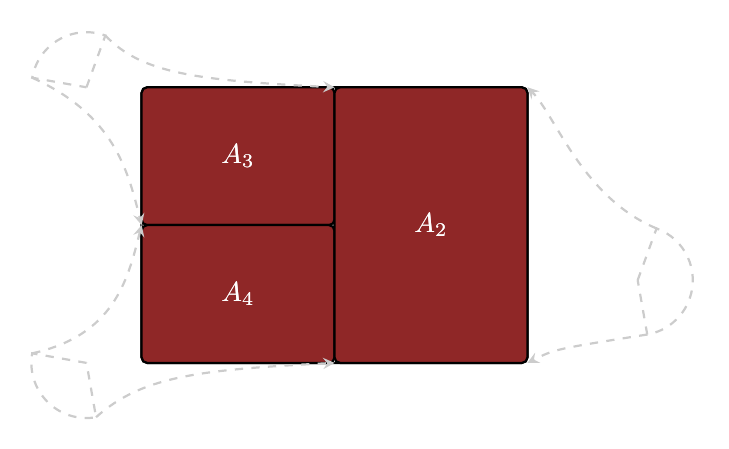
\begin{tikzpicture}[scale=0.35, thick]
  \draw [rounded corners=2pt, color=black] (4, 0) rectangle +(14, 10);
  %\node at (14.5, -1) { $\quad \mathbb{P}_{\pi}[ A_{3} ] + \mathbb{P}_{\pi}[ A_{4} ] + \mathbb{P}_{\pi}[ A_{2} ]$ };
  %\node at (14.5, -2.5) { $= \quad\quad \mathbb{P}_{\pi}[ A_{1} ] \quad\quad + \mathbb{P}_{\pi}[ A_{2} ]$ };
  %\node at (14.5, -4) { $= \quad\quad\quad\quad\;\, \mathbb{P}_{\pi}[ X ] \quad\quad\quad\quad$ };
  %\node at (14.5, -5.5) { $= \quad\quad\quad\quad\quad\; 1 \quad\quad\quad\quad\quad\;$ };

  \fill [rounded corners=2pt, color=dark, text=white] (4, 5) rectangle +(7, 5) node[midway] { $A_{3}$ }; 
  \draw [rounded corners=2pt, color=black, text=white] (4, 5) rectangle +(7, 5) node[midway] { $A_{3}$ }; 
  
  \fill [rounded corners=2pt, color=dark, text=white] (4, 0) rectangle +(7, 5) node[midway] { $A_{4}$ };
  \draw [rounded corners=2pt, color=black, text=white] (4, 0) rectangle +(7, 5) node[midway] { $A_{4}$ };
  
  \fill [rounded corners=2pt, color=dark, text=white] (11, 0) rectangle +(7, 10) node[midway] { $A_{2}$ };
  \draw [rounded corners=2pt, color=black, text=white] (11, 0) rectangle +(7, 10) node[midway] { $A_{2}$ };
  
  \draw[color=gray80, dashed] (2, 10) -- ({2 + 2 * sin(20)}, {10 + 2 * cos(20)}) arc (70:170:2) -- (2, 10);
  
  \draw [->, >=stealth, color=gray80, dashed] ({2 + 2 * sin(20)}, {10 + 2 * cos(20)}) .. controls (4, 10.5) and (6, 10.25) .. (11, 10);
  \draw [->, >=stealth, color=gray80, dashed] ({2 - 2 * cos(10)}, {10 + 2 * sin(10)}).. controls (3, 9) and (3.5, 7) .. (4, 5);
  
  \draw[color=gray80, dashed] (2, 0) -- ({2 - 2 * cos(10)}, {0 + 2 * sin(10)}) arc (170:280:2) -- (2, 0);  
  
  \draw [->, >=stealth, color=gray80, dashed] ({2 - 2 * cos(10)}, {0 + 2 * sin(10)}) .. controls (3, 1) and (3.5, 3) .. (4, 5);
  \draw [->, >=stealth, color=gray80, dashed] ({2 + 2 * sin(10)}, {0 - 2 * cos(10)}).. controls (4, -0.5) and (6, -0.25) .. (11, 0);
  
  \draw[color=gray80, dashed] (22, 3) -- ({22 + 2 * sin(20)}, {3 + 2 * cos(20)}) arc (70:-80:2) -- (22, 3);
  
  \draw [->, >=stealth, color=gray80, dashed] ({22 + 2 * sin(20)}, {3 + 2 * cos(20)}) .. controls (20, 6) and (19, 9) .. (18, 10);
  \draw [->, >=stealth, color=gray80, dashed] ({22 + 2 * sin(10)}, {3 - 2 * cos(10)}).. controls (19, 0.5) .. (18, 0);
\end{tikzpicture}

\end{document}  